Crear la base de datos \emph{universidad} en \textit{Mongo Shell}:

\begin{figure}[H]
  \centering
  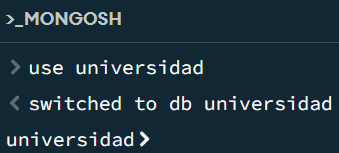
\includegraphics{Imagenes/parte1/1.1.png}
  \caption{Creación de la base de datos universidad}
\end{figure}

Crear la colección \emph{`estudiantes'}:

\begin{figure}[H]
  \centering
  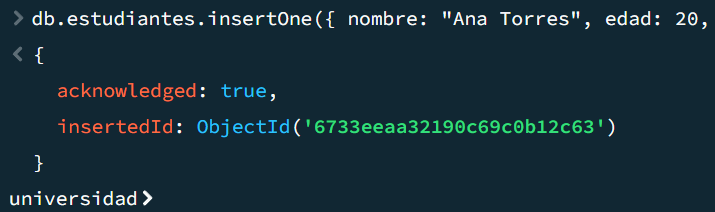
\includegraphics[scale = 0.8]{Imagenes/parte1/1.2.png}
  \caption{Creación de la colección estudiantes}
\end{figure}

Crear la colección \emph{`cursos'}:

\begin{figure}[H]
  \centering
  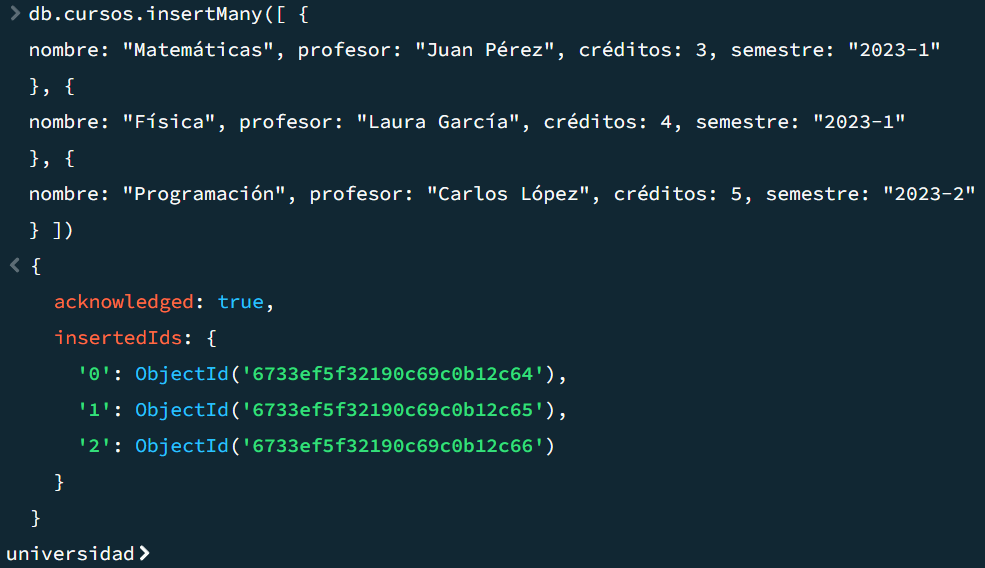
\includegraphics[scale = 0.5]{Imagenes/parte1/1.3.png}
  \caption{Creación de la colección cursos}
\end{figure}